\documentclass{ximera}


\begin{document}
    % Start specifieke settings:   
    \author{Zomercursus KU Leuven}
    \xmtitle{Machten van complexe getallen: formule van De Moivre}{}
    % Start inhoud ximera
     
    \label{xim:complexe_getallen_demoivre}
 

% LABEL AND AUTHOR MOET NOG WORDEN AANGEPAST 



De n-de macht van een complexe getal \(z^n\) is het n-voudig product \(z \cdot z \cdot z \cdot \dots \cdot z \). (n-keer invoegen). Met de vermenigvuldiging van complexe getallen kan dit n-voudig product uitgerekend worden. Ook hier zijn de berekeningen met de goniometrische schrijfwijze veel eenvoudiger. 

Het meest eenvoudige geval \(n=2\) is het kwadraat \(z^2\) van een complex getal. Dit is de vermenigvuldiging van het complex getal met zichzelf. Voor een complex getal \(z\) met als goniometrische schrijfwijze \(r(\cos \theta + i \sin \theta ) \) wordt dit: 

\[
z^2 = z \cdot z  = r(\cos \theta + i \sin \theta ) \cdot r(\cos \theta + i \sin \theta ) = r^2(\cos (\theta + \theta) + i \sin (\theta + \theta) ) =  r^2(\cos 2\theta + i \sin 2\theta ). 
\]

Het herhalen van deze methode levert dan hogere machten van een complex getal.  \(z^3 = z^2 \cdot z \). Het algemene resultaat staat bekend als de formule van DeMoivre: 
 
\begin{proposition}[Formule van De Moivre]\nl 
Voor een complex getal $z= r (\cos \theta + i \sin \theta )$ en elk natuurlijk getal $n$ geldt
\[
z^n = r^n(\cos n\theta + i \sin n\theta )
\]
\end{proposition}
 
\begin{example}
    We kunnen $(1+i)^8$ op 2 manieren berekenen:         
        \begin{enumerate}
            \item $(1+i)(1+i)=1+2i-1=2i$, dus $(1+i)(1+i)(1+i)(1+i)=(2i)^2=-4$, dus $(1+i)^8=(-4)^2=16$
            \item $1+i=\sqrt{2}(\cos \frac{\pi}{4}+i\sin\frac{\pi}{4})$, dus $(1+i)^8=(\sqrt{2})^8(\cos  \frac{8\pi}{4}+i\sin \frac{8\pi}{4})=2^4(\cos 2\pi +i \sin 2\pi)=16(1+i\cdot 0)=16$
        \end{enumerate}
         
    \end{example}
 
\begin{exercise} Bereken met de formule van De Moivre
    \begin{question} $(\sqrt 3 + i)^3 = \answer[onlineshowanswerbutton]{8i}$
    \end{question}
    \begin{question} $(-1-i)^{20} = \answer[onlineshowanswerbutton]{-1024}$
    \end{question}
    \begin{question} $(1+ i)^{21} = \answer[onlineshowanswerbutton]{-1024-1024i}$
    \end{question}
    \begin{question} $(-\sqrt 3 + i)^5 = \answer[onlineshowanswerbutton]{16\sqrt3+16i}$
    \end{question}
\end{exercise}


\begin{exercise}
    Gegeven is het complex getal \(z = \cos\frac{3\pi}{4} + i\sin\frac{3\pi}{4}\). 
    \begin{question}
        Bereken \(z^0, z^1, z^2, z^3, \dots, z^8 \) en schrijf telkens het resultaat in cartesische vorm. 
        \begin{oplossing}\nl
            Het getal \(z\) ligt op de eenheidscirkel (\(r=1\)) met argument \(\frac{3\pi}{4}\). Volgens de formule van De Moivre geldt voor elke natuurlijke exponent \(n\):
            \[
                z^n = \cos\frac{3n\pi}{4} + i\sin\frac{3n\pi}{4}\,.
            \]
            Omdat \(\cos\frac{3\pi}{4}=\sin\frac{3\pi}{4}=-\frac{\sqrt{2}}{2}\), \(\cos\frac{\pi}{4}=\sin\frac{\pi}{4}=\frac{\sqrt{2}}{2}\) en \(\cos\frac{\pi}{2}=0\), \(\sin\frac{\pi}{2}=1\), vind je in cartesische vorm:
            \begin{align*}
                z^0 &= 1, &
                z^1 &= -\frac{\sqrt{2}}{2}+\frac{\sqrt{2}}{2}\,i, &
                z^2 &= -i, \\
                z^3 &= \frac{\sqrt{2}}{2}+\frac{\sqrt{2}}{2}\,i, &
                z^4 &= -1, &
                z^5 &= \frac{\sqrt{2}}{2}-\frac{\sqrt{2}}{2}\,i, \\
                z^6 &= i, &
                z^7 &= -\frac{\sqrt{2}}{2}-\frac{\sqrt{2}}{2}\,i, &
                z^8 &= 1\,.
            \end{align*}
        \end{oplossing}
    \end{question}
    \begin{question}
        Stel de opeenvolgende machten van \(z\) voor in het complexe vlak. Wat valt je op? 
        \begin{oplossing}\nl
            Alle punten liggen op de eenheidscirkel. Bij elke verhoging van de exponent met \(1\) roteert het beeldpunt over een vaste hoek \(\frac{3\pi}{4}\) rond de oorsprong (vermenigvuldigen met \(z\) is dus een rotatie over \(135^\circ\)). Na acht stappen ben je terug bij \(z^8=1=z^0\): de acht punten vormen een regelmatige achthoek op de cirkel (de machten herhalen zich met periode \(8\) omdat \(8\cdot\frac{3\pi}{4}=6\pi\) een veelvoud van \(2\pi\) is).

            \begin{image}[0.85\textwidth]
                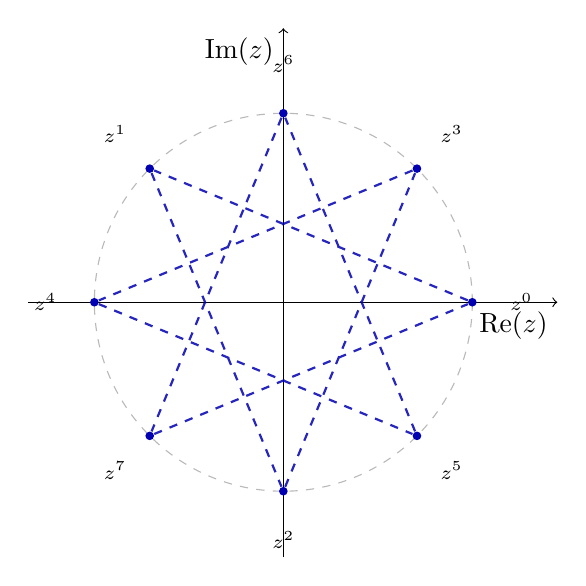
\begin{tikzpicture}[scale=2.4]
                    \draw[->] (-1.35,0) -- (1.45,0) node[below left] {Re$(z)$};
                    \draw[->] (0,-1.35) -- (0,1.45) node[below left] {Im$(z)$};
                    \draw[gray!55, dashed] (0,0) circle (1);
                    \foreach \n in {0,...,7} {
                        \pgfmathsetmacro{\hoek}{135*\n}
                        \node[circle, fill=blue!70!black, inner sep=1.1pt] (Z\n) at ({\hoek}:1) {};
                        \node[font=\scriptsize, inner sep=0.5pt] at ({\hoek}:1.26) {$z^{\n}$};
                    }
                    \draw[blue!70!black, thick, dashed, opacity=0.85]
                        (Z0) -- (Z1) -- (Z2) -- (Z3) -- (Z4) -- (Z5) -- (Z6) -- (Z7) -- (Z0);
                \end{tikzpicture}
            \end{image}
        \end{oplossing}
    \end{question}
\end{exercise}






% NOG INVOEGEN OP MAAT; EEN MEER UITGEBREIDE  BESPREKEING VAN DE MEETKUNDIGE BETEKENIS ZIE KOEN; HIERVOOR IS GEOGEBRA EN KENNISCLIP OOK GESCHIKT. 


 
 
\end{document}